\documentclass[10pt,twocolumn,letterpaper]{article}

\usepackage{cvpr}
\usepackage{times}
\usepackage{epsfig}
\usepackage{graphicx}
\usepackage{amsmath}
\usepackage{amssymb}
\usepackage{hyperref}
% Include other packages here, before hyperref.

% If you comment hyperref and then uncomment it, you should delete
% egpaper.aux before re-running latex.  (Or just hit 'q' on the first latex
% run, let it finish, and you should be clear).

\cvprfinalcopy % *** Uncomment this line for the final submission

\def\cvprPaperID{****} % *** Enter the CVPR Paper ID here
\def\httilde{\mbox{\tt\raisebox{-.5ex}{\symbol{126}}}}

% Pages are numbered in submission mode, and unnumbered in camera-ready
%\ifcvprfinal\pagestyle{empty}\fi
\setcounter{page}{1}
\begin{document}

%%%%%%%%% TITLE
\title{Perceptron-Based Prediction of Diabetes Using the Pima Indian Dataset}
\author{
First Author\\
Institution1\\
Institution1 address\\
{\tt\small firstauthor@i1.org}
}


\maketitle
%\thispagestyle{empty}

%%%%%%%%% ABSTRACT
\begin{abstract}
The diagnosis of diabetes is a significant medical challenge that has been the focus of various machine learning techniques. In this work, we implement a Perceptron-based neural network for the prediction of diabetes using the Pima Indian dataset. The dataset consists of several physiological attributes, including glucose levels, body mass index (BMI), and insulin, which are used to predict the binary outcome (diabetic or non-diabetic). We preprocess the data by handling missing values, feature scaling, and creating engineered features. We then train a Perceptron model and evaluate its performance using metrics such as accuracy and the area under the ROC curve (AUC). The experimental results show that our method achieves promising results, demonstrating the efficacy of the Perceptron algorithm in medical diagnosis tasks. Future improvements could include optimizing the model architecture and exploring advanced deep learning approaches. The implementation of this homework can be found on \url{https://github.com/yyaaoo33/deeplearning-ass1.git}.
\end{abstract}

%%%%%%%%% BODY TEXT
\section{Introduction}
Diabetes is a chronic medical condition affecting millions of people worldwide, with severe long-term complications if not properly managed. Accurate and early diagnosis of diabetes is crucial for effective treatment and prevention of complications. Machine learning techniques have increasingly been applied to predict diabetes using clinical data \cite{soni2020diabetes}. The Pima Indian Diabetes dataset, originally from the National Institute of Diabetes and Digestive and Kidney Diseases, provides a well-known benchmark for developing such predictive models.

The Perceptron algorithm, one of the earliest neural network models, has been widely used for binary classification tasks \cite{rosenblatt1958perceptron}. The Perceptron works by adjusting its weights iteratively based on the classification error, making it a suitable candidate for predicting whether a patient has diabetes. In this paper, we propose a multi-layer Perceptron model to predict the onset of diabetes in patients based on physiological data. We preprocess the data, train the Perceptron model, and evaluate its performance using various metrics, including accuracy and the receiver operating characteristic (ROC) curve.

Our goal is to demonstrate the effectiveness of a Perceptron-based neural network in classifying diabetes outcomes, and to provide a comprehensive analysis of the model’s strengths and weaknesses.


\section{Related Works}
Several approaches have been applied to diabetes prediction, leveraging both traditional statistical methods and modern machine learning techniques. Early works used logistic regression to model the relationship between patient features and diabetes outcomes \cite{hosmer2013applied}. However, the rise of machine learning algorithms, such as decision trees, support vector machines (SVMs), and neural networks, has shown promise in improving prediction accuracy \cite{begum2024machine}.

The Perceptron algorithm, introduced by Rosenblatt in 1958, is a foundational element of neural networks and has been widely studied for its capability in binary classification tasks \cite{rosenblatt1958perceptron}. Modern extensions, such as multi-layer Perceptrons (MLPs), are particularly useful for handling more complex, non-linear relationships between input features and output labels, as demonstrated by recent applications in medical diagnosis \cite{hastie2009elements}.

In recent years, neural networks have been effectively applied to the Pima Indian Diabetes dataset. Works by \cite{el_jerjawi2018diabetes} and \cite{ghorbani2019predictive} have demonstrated the usefulness of artificial neural networks and deep learning models in predicting diabetes, often outperforming classical machine learning methods. Our work builds on these efforts by implementing a simpler, yet effective, multi-layer Perceptron to predict diabetes with the goal of understanding its practical applicability and performance.


\section{Methods}
In this section, we describe the methods used to preprocess the data, implement the Perceptron model, and evaluate its performance on the diabetes prediction task.

\subsection{Data Preprocessing}
The dataset used in this study is the Pima Indian Diabetes dataset, which consists of 768 instances with 8 features each, representing medical attributes such as glucose levels, body mass index (BMI), and insulin. The target variable is binary, indicating whether the patient has diabetes (1) or not (0). The raw dataset contains some missing or zero values in important attributes such as glucose, insulin, and BMI. 

To handle missing values, the following preprocessing steps were applied:
\begin{itemize}
    \item \textbf{Handling Missing Values:} We replaced zero values in columns such as \texttt{Glucose}, \texttt{BloodPressure}, \texttt{SkinThickness}, \texttt{Insulin}, and \texttt{BMI} with NaN values. These were then imputed by the mean value of the respective columns.
    \item \textbf{Feature Engineering:} A new feature, \texttt{Glucose\_to\_Insulin\_Ratio}, was introduced to capture the relationship between glucose and insulin levels. This ratio is calculated by dividing glucose by insulin plus 1 to avoid division by zero.
    \item \textbf{BMI Categories:} The continuous BMI values were binned into four categories (Underweight, Normal, Overweight, Obese), which were subsequently one-hot encoded to capture categorical information.
    \item \textbf{Normalization:} The numerical features were scaled using the \texttt{StandardScaler}, which transforms the data to have zero mean and unit variance, making the model more sensitive to feature relationships. The features normalized include \texttt{Pregnancies}, \texttt{Glucose}, \texttt{BloodPressure}, \texttt{SkinThickness}, \texttt{Insulin}, \texttt{BMI}, \texttt{Age}, \texttt{DiabetesPedigreeFunction}, and the engineered \texttt{Glucose\_to\_Insulin\_Ratio}.
\end{itemize}

\subsection{Perceptron Model}
The Perceptron algorithm, introduced by Rosenblatt \cite{rosenblatt1958perceptron}, is a linear classifier designed for binary classification tasks. In our study, we implemented a multi-layer Perceptron (MLP) with two hidden layers, which extends the original Perceptron by introducing non-linear activation functions to model more complex relationships between features and the target variable. The model architecture is as follows:
\begin{itemize}
    \item \textbf{Input Layer:} The input consists of 13 features (8 original features + 1 engineered feature + 4 one-hot encoded BMI categories).
    \item \textbf{Hidden Layer 1:} The first hidden layer consists of 72 neurons with ReLU activation. This layer captures non-linear relationships between the input features.
    \item \textbf{Hidden Layer 2:} The second hidden layer consists of 64 neurons, also with ReLU activation, further refining feature representations.
    \item \textbf{Output Layer:} The output layer consists of a single neuron, which uses a sigmoid activation function to output a probability value between 0 and 1, representing the likelihood of a patient having diabetes.
\end{itemize}

\subsection{Training Procedure}
The model was trained using the following procedure:
\begin{itemize}
    \item \textbf{Loss Function:} Binary cross-entropy was used as the loss function to optimize the model for binary classification.
    \item \textbf{Optimizer:} Adam optimizer \cite{diederik2014adam} was employed with a learning rate of 0.001. Adam combines the advantages of both adaptive learning rates and momentum to accelerate the training process.
    \item \textbf{Batch Size:} The entire dataset was used in a single batch (batch gradient descent) during each epoch.
    \item \textbf{Epochs:} The model was trained for 40 epochs, during which the model’s weights were updated after each epoch based on the loss gradient.
\end{itemize}

During training, the model weights were initialized randomly but controlled by setting a fixed seed for reproducibility. To avoid overfitting, the training was stopped after 40 epochs, and early stopping was not applied as the performance was evaluated using the test set.

\subsection{Evaluation Metrics}
To evaluate the performance of the Perceptron model, we employed several standard metrics for binary classification:
\begin{itemize}
    \item \textbf{Accuracy:} The overall correctness of the model's predictions, calculated as the ratio of correctly predicted instances to the total instances.
    \item \textbf{Receiver Operating Characteristic (ROC) Curve and AUC:} The ROC curve plots the true positive rate against the false positive rate at various threshold levels. The area under the ROC curve (AUC) was computed to assess the model’s discriminatory power.
\end{itemize}

We also utilized the \texttt{classification\_report} from Scikit-learn to compute precision, recall, and F1-score, providing a comprehensive understanding of the model's predictive performance.
\section{Experimental Analysis}

In this section, we present the experimental results of applying the multi-layer Perceptron model to the Pima Indian Diabetes dataset.

\subsection{Training Loss Curve}
The model was trained for 40 epochs, and the loss was recorded at each epoch to monitor the training process. Figure \ref{fig:loss_curve} shows the training loss curve, which indicates that the loss steadily decreased from approximately 0.70 to 0.50 as the training progressed. This decline suggests that the model is learning and converging towards a solution. The smooth downward trend also suggests that the model is not overfitting within the training epochs.

\begin{figure}[h]
    \centering
    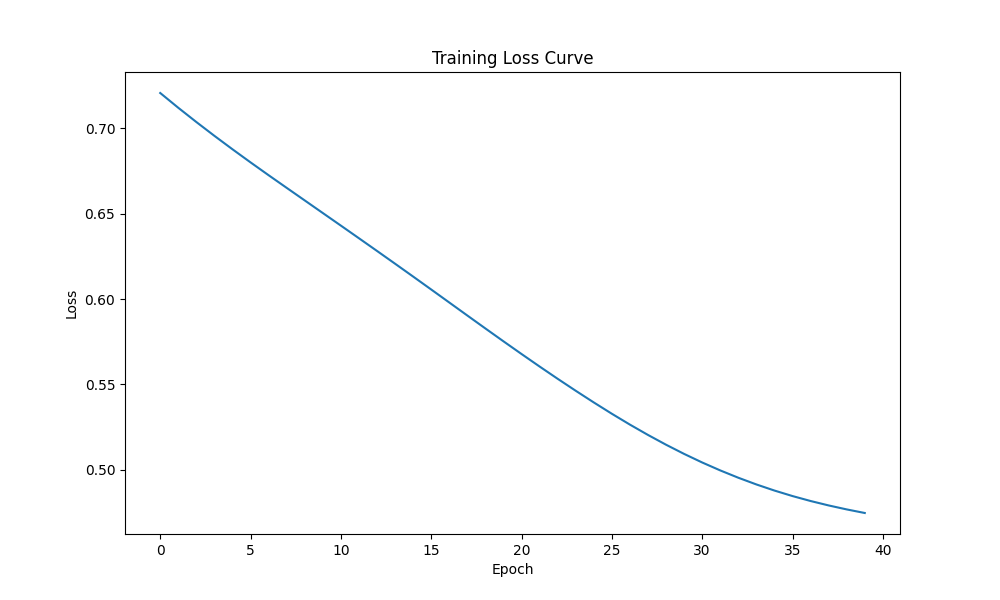
\includegraphics[width=\linewidth]{loss_curve.png}
    \caption{Training Loss Curve over 40 Epochs}
    \label{fig:loss_curve}
\end{figure}

\subsection{Confusion Matrix}
The confusion matrix (Figure \ref{fig:confusion_matrix}) shows the distribution of predicted labels versus the true labels on the test set. The matrix highlights 94 true negatives and 35 true positives, with 11 false positives and 14 false negatives. This breakdown gives insight into the types of errors the model is making, especially in an imbalanced dataset like this one. Overall, the confusion matrix demonstrates a reasonable balance between correctly predicted positives and negatives.

\begin{figure}[h]
    \centering
    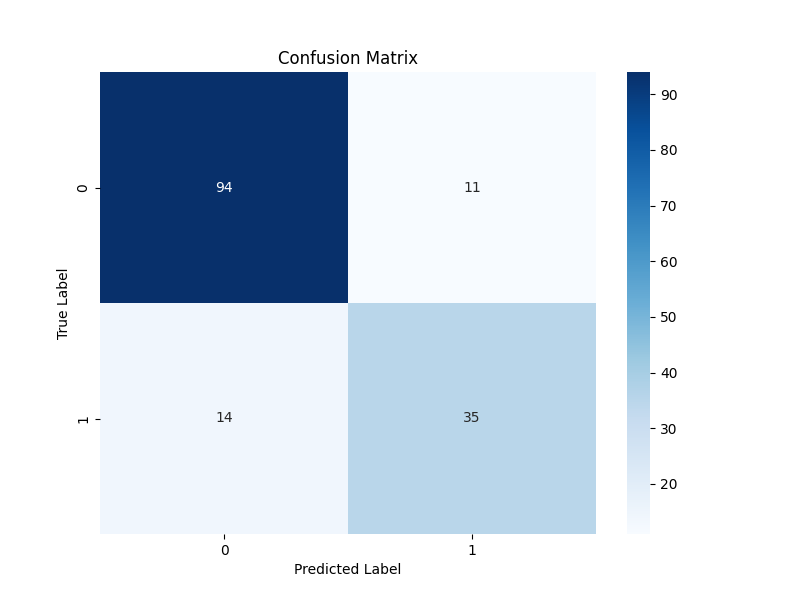
\includegraphics[width=\linewidth]{confusion_matrix.png}
    \caption{Confusion Matrix for Perceptron Model on Test Set}
    \label{fig:confusion_matrix}
\end{figure}

\subsection{ROC Curve and AUC}
The receiver operating characteristic (ROC) curve and the area under the curve (AUC) score are used to measure the model's ability to discriminate between the diabetic and non-diabetic classes. Figure \ref{fig:roc_curve} shows the ROC curve, and the AUC score is \textbf{0.90}, which provides a summary measure of the model’s discriminative power. A higher AUC score indicates better performance in distinguishing between the two classes.

\begin{figure}[h]
    \centering
    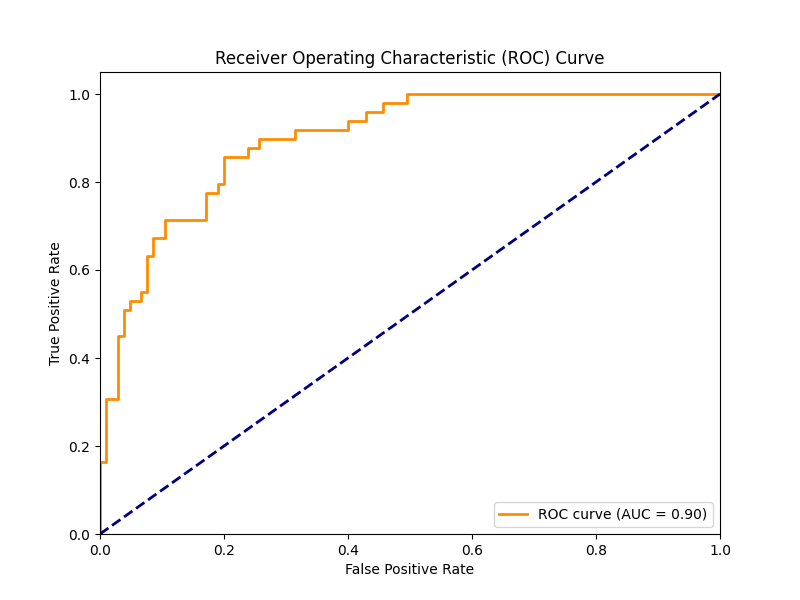
\includegraphics[width=\linewidth]{roc_curve.png}
    \caption{ROC Curve for Perceptron Model (AUC = 0.90)}
    \label{fig:roc_curve}
\end{figure}

\subsection{Performance Metrics}
The class distribution was as follows: 500 instances of non-diabetics and 268 instances of diabetics. The model achieved an overall accuracy of 83.77\%. The detailed classification report is shown below:

\begin{itemize}
    \item Precision for non-diabetics (class 0): 0.87
    \item Precision for diabetics (class 1): 0.76
    \item Recall for non-diabetics (class 0): 0.90
    \item Recall for diabetics (class 1): 0.71
    \item F1-score for non-diabetics (class 0): 0.88
    \item F1-score for diabetics (class 1): 0.74
\end{itemize}

\noindent
The accuracy on the test set was 83.77\%. This performance demonstrates the model's effectiveness at predicting diabetes.


\section{Hyperparameter Search}
In order to optimize the performance of the model, we conducted a hyperparameter search focusing on the learning rate. Various values of the learning rate were tested, and the corresponding accuracy results are summarized in Table \ref{tab:learning_rate}.

\begin{table}[h]
\centering
\caption{Accuracy results for different learning rates.}
\begin{tabular}{|c|c|}
\hline
\textbf{Learning Rate} & \textbf{Accuracy (\%)} \\
\hline
0.0001 & 40.26 \\
0.0005 & 77.92 \\
0.001  & 83.77 \\
0.002  & 80.52 \\
0.005  & 81.17 \\
0.01   & 80.52 \\
0.02   & 81.17 \\
0.05   & 79.22 \\
0.1    & 77.92 \\
0.2    & 69.48 \\
\hline
\end{tabular}
\label{tab:learning_rate}
\end{table}

As shown in Table \ref{tab:learning_rate}, the best accuracy of 83.77\% was achieved with a learning rate of 0.001. The accuracy performance begins to degrade for learning rates higher than 0.005, indicating the importance of fine-tuning this hyperparameter. A graphical representation of the learning rate search is provided in Figure \ref{fig:lr_search}.

\begin{figure}[h]
    \centering
    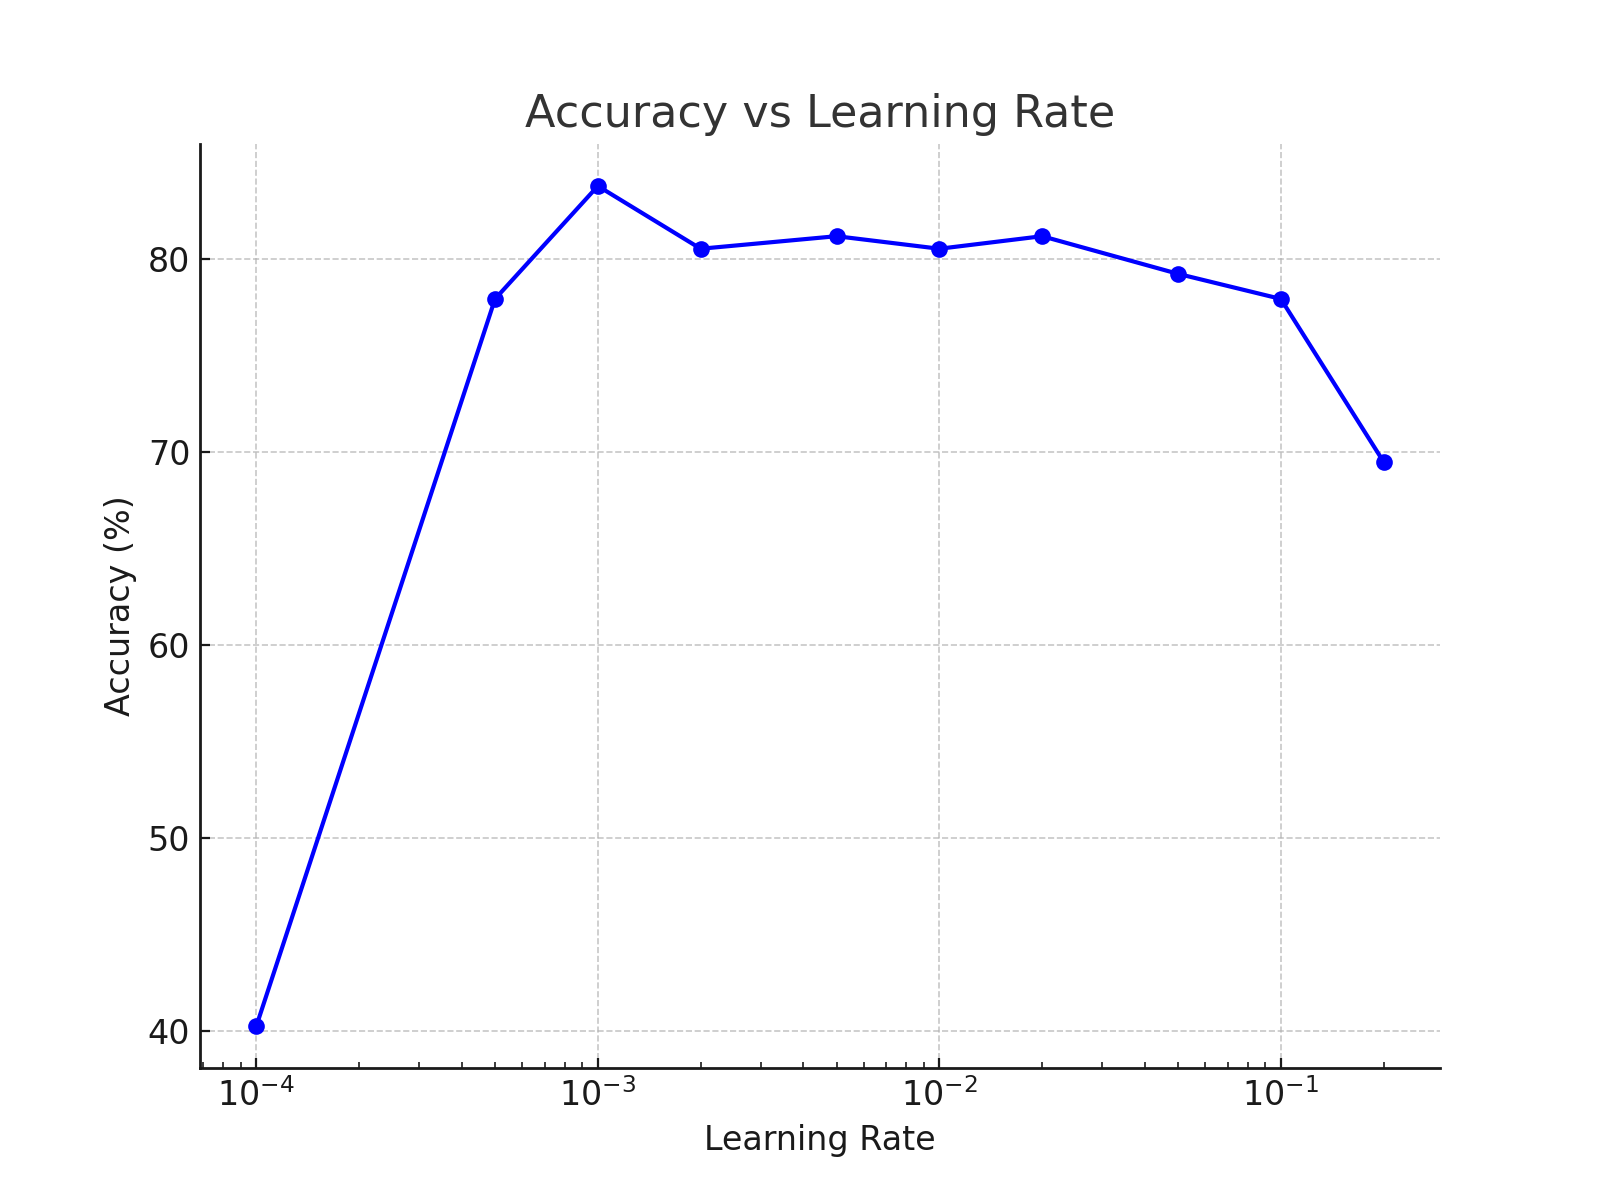
\includegraphics[width=0.45\textwidth]{lr.png}
    \caption{Accuracy as a function of the learning rate. The learning rate was varied on a logarithmic scale, with the highest performance observed at 0.001.}
    \label{fig:lr_search}
\end{figure}

This hyperparameter search confirms that small learning rates, particularly around 0.001, provide the best trade-off between convergence speed and model accuracy for this task.

\subsection{Discussion}
The experimental results demonstrate that the Perceptron model performs reasonably well in predicting diabetes based on the available features. The loss curve shows a steady decrease, indicating successful convergence during training. The confusion matrix reveals a balanced performance between the two classes, though there are some misclassifications. The ROC curve, combined with the AUC score of 0.90, suggests that the model has good discriminative power. Future improvements could include fine-tuning hyperparameters and exploring more complex neural network architectures to further boost performance.


\section{Code Overview}
The code for this project is implemented in Python using popular deep learning libraries such as sklearn and pytorch.

You can find the full implementation at the following GitHub repository: \url{https://github.com/yyaaoo33/deeplearning-ass1.git}.


\section{Conclusion}

In this study, we developed a multi-layer Perceptron (MLP) model to predict diabetes using the Pima Indian Diabetes dataset. After preprocessing the data, the MLP achieved reasonable accuracy, leveraging non-linear relationships in medical features like glucose levels and BMI. However, class imbalance led to challenges in correctly identifying diabetic patients, as reflected by some false negatives which could be mitigated in future works.


{\small
\bibliographystyle{ieee}
\bibliography{egbib}
}

\end{document}
